\documentclass[oneside,a4paper,spanish,links]{amca}
%
\usepackage{graphicx}
\usepackage{amsmath,amsfonts}

\title{VOLUME RENDERING APLICADO A LA RENDERIZACION DE PANES EN TIEMPO REAL}

\author[a]{Rodrigo Baravalle}
\author[b]{Leonardo Scandolo}
\author[c]{Claudio Delrieux}
\author[d]{Cristian G. Bauza}
\author[a]{Juan C. G\'omez}
%
\affil[a]{Laboratorio de Sistemas Din\'amicos y Procesamiento de Se\~nales, FCEIA, Universidad Nacional de Rosario, CIFASIS-CONICET,
  Ocampo y Esmeralda, S2000EZP~Rosario, Argentina,
  baravalle@cifasis-conicet.gov.ar, \url{http://www.cifasis-conicet.gov.ar/grupo4.html}}
%
\affil[b]{Departamento de Ciencias de la Computaci\'on, FCEIA, Universidad Nacional de Rosario,
  Pellegrini 250, 2000~Rosario, Argentina,
  leonardo@fceia.unr.edu.ar, \url{http://web.fceia.unr.edu.ar/es/institucional/escuelas/118-departamento-ciencias-de-la-computacion-ecen.html}}

\affil[c]{Departamento de Ingenier\'ia El\'ectrica y de Computadoras, Universidad Nacional del Sur - IIIE-CONICET,
  Col\'on 80, 8000FTN~Bah\'ia Blanca, Argentina,
  cad@uns.edu.ar, \url{http://www.ingelec.uns.edu.ar/}}

\affil[d]{Instituto de Investigaci\'on PLADEMA- Facultad de Ciencias Exactas - Universidad Nacional del Centro, Campus Universitario,
  Paraje Arroyo Seco, (B7001BBO) Tandil, Buenos Aires, Argentina
  crgarcia@exa.unicen.edu.ar, \url{http://www.exa.unicen.edu.ar/es/d_investigacion/inst_pladema/index.html}}


%% NOTE: IF ALL AUTHORS BELONG TO THE SAME AFFILIATION
%% USE THE `\voidaffil' MACRO FOR THE AFFILIATION CODE.
%% Example:
%% \author[\voidaffil]{First A. Author}
%% \author[\voidaffil]{Second B. Author}
%% \author[\voidaffil]{Third C. Author}
%% \author[\voidaffil]{Fourth D. Author}
%% %
%% \affil[\voidaffil]{Grupo de Mec\'anica Computacional,
%% Universidad Nacional de Villa Carolina,
%% Los Alerces 3492, 4200 Villa Carolina, Argentina,
%% gmc@uncarolina.edu.ar, http://www.uncarolina.edu.ar/gmc}

\begin{document}
\vspace{3cm}

\maketitle

%% To set PDF METADATA: uncomment and replace fields in
%% UPPERCASE with appropriate values. 
%% 
%% \hypersetup{
%%   pdfauthor={AUTHORS},
%%   pdfkeywords={KEYWORDS},
%%   pdftitle={TITLE}
%% }
%%
%% For instance
%% \hypersetup{
%%   pdfauthor={Sponge B. and Star P.},
%%   pdfkeywords={multiphase flow, air-liquid mixtures},
%%   pdftitle={A new model for multi-phase flow}
%% }
%%
%% NOTE: To set the metadata is recommended but not absolutely
%% neccesary. 
%% This was done before with the \pdfinfo command,
%% but according to this post:
%% http://de.nntp2http.com/comp/text/tex/2008/12/5358fd061de9703a781885a5dcf98364.html
%% if `hyperref' is used, then you must use \hypersetup{} not \pdfinfo{}

\begin{keywords}
  Direct Volume Rendering, Pan, Tiempo Real.
\end{keywords}

\begin{abstract}
  El modelado foto-real\'istico de materiales con una estructura interna compleja presenta un desaf\'io en Computaci\'on Gr\'afica. Espec\'ificamente, la miga del pan es un material transl\'ucido cuya estructura es porosa, mostrando detalles en distintas escalas. Si se pretende obtener resultados foto-realistas, deben modelizarse fen\'omenos tales como sombras internas, oclusi\'on, transmitancia y absorci\'on. La soluci\'on t\'ipica en estos casos es la aplicaci\'on directa de la ecuaci\'on del rendering, es decir, utilizar iluminaci\'on global (ray tracing, path tracing). Sin embargo, estos m\'etodos presentan un costo computacional elevado y necesitan una malla 3D detallada del material.

El estado del arte en renderizaci\'on de materiales porosos utiliza un complejo procedimiento de captura donde la luz que es reflejada por el material es obtenida en distintos \'angulos. Esa informaci\'on es utilizada para reconstruir un modelo computacional del material. Si bien utilizando esta t\'ecnica es posible modelar alguna de las propiedades lum\'inicas deseadas, los costos computacionales asociados, el procedimiento de captura requerido y la baja variabilidad de la imagen resultante han provocado una dificultosa aplicaci\'on pr\'actica del m\'etodo.


En este trabajo proponemos el estudio e implementaci\'on en GPU de un modelo basado en direct volume rendering sobre un campo escalar representando la estructura de la miga de pan sin utilizar estructuras intermedias. Las im\'agenes obtenidas muestran resultados promisorios en tiempo real. La miga es representada a trav\'es de un campo escalar 3D, el cual es computado en dos pasos. El primero utiliza una generaci\'on a trav\'es de sistemas de part\'iculas, y el segundo aplica sistemas din\'amicos para evolucionar las part\'iculas, imitando el proceso de leudado y cocci\'on del pan.

\end{abstract}

\section{INTRODUCCION}

La apariencia de la miga de pan y otros materiales cocidos, como pizzas y budines, ha sido considerada un desaf\'io para renderizar debido a la compleja interacci\'on del material con la luz. Los costos computacionales asociados (almacenamiento de memoria y tiempo computacional) de estos procesos f\'isicos hacen que el rendering sea impr\'actico en aquellas areas donde la interactividad sea mandatoria. El crecimiento exponencial en poder de c\'omputo, provocado mayormente por el dise\~no masivamente paralelo de las placas gr\'aficas \citep{Yeo09,Harris06}, ha hecho posible simular algunos fen\'omenos de la luz mencionados en tiempos computacionales aceptables, sin embargo el campo es a\'un objeto de estudio \citep{Voglsam2013}.

La geometr\'ia observable en estos materiales representa de por s\'i un desaf\'io extra. Estas estructuras porosas son el resultado de complejos mecanismos que involucran deformaciones f\'isicas y reacciones qu\'imicas. La producci\'on de pan presenta dos etapas: leudado y cocci\'on. Durante el leudado, la levadura genera $CO_{2}$, produciendo burbujas en la masa \citep{Shah1998}. El proceso de cocci\'on \citep{Mondal2008} modifica estas burbujas de distintas maneras \citep{Scanlon2001}, d\'andole al pan su estructura final. Se han hecho intentos de s\'intesis de esta estructura \citep{Cho2007}, pero el resultado es en realidad un proceso art\'istico. En este trabajo proponemos la utilizaci\'on de sistemas din\'amicos \citep{Strogatz2001} aplicados a la evoluci\'on de sistemas de part\'iculas \citep{Reeves83}, utilizando un trabajo que los autores realizaron previamente \citep{Baravalle2011}. Estos esfuerzos son un intento de imitar el leudado y la cocci\'on mencionados. Procesos complejos como el clima y determinados fluidos son explicados por medio del uso de ecuaciones diferenciales que desciben su comportamiento y apariencia. Esta idea es utilizada en este trabajo para modelar el crecimiento de burbujas en el interior de panes. El proceso arroja como resultado una estrucura similar a burbujas sobre un fluido, lo cual puede observarse en distintos panes. Otros trabajos computan el valor de la textura en cada voxel del dominio \citep{Perlin1989}, por lo cual no requieren memoria para alojar la textura 3D. El enfoque estad\'istico requerido en estos m\'etodos resulta inadecuado para capturar la distribuci\'on de burbujas.

La renderizaci\'on de estas estructuras depende fuertemente de la estructura de datos utilizada para representarlas. Si una malla tradicional 3D es utilizada, la misma debe computarse a partir de un campo escalar previamente construido, utilizando t\'ecnicas como 
marching cubes \citep{Lorensen1987}. Este proceso podr\'ia no resultar trivial debido a la estructura porosa del material. La representaci\'on de la miga de pan como una superficie resulta tambi\'en inadecuada, ya que existen estructuras (burbujas) sobre la misma, por lo cual soluciones t\'ipicas como utilizar funciones bidireccionales de distribuci\'on de reflectancia (BRDF) \citep{Kurt2009} no son factibles. Una compleja soluci\'on es propuesta \citep{Tong2005}, pero el dif\'icil proceso de captura asociado, junto con la baja variabilidad en las im\'agenes resultantes y los costos computacionales del m\'etodo, han hecho que el mismo no sea utilizado de manera masiva. 

En este trabajo se propone la aplicaci\'on de Direct Volume Rendering (DVR) \citep{Levoy1988, Kratz2006} sobre un campo escalar para renderizar el interior de distintos objetos cocidos. El proceso de DVR consiste en lanzar rayos desde una c\'amara virtual hacia el campo escalar, acumulando distintas propiedades para cada pixel. El m\'etodo no utiliza estructuras intermedias, simplificando el proceso de modelado. La forma exterior del material puede ser definida en tiempo real en la GPU, haciendo posible realizar cortes y deformaciones a la miga original. Adem\'as, la corteza del mismo puede ser establecida utilizando funciones de transferencia (definici\'on de distintas regiones en el espacio). Resultados satisfactorios son obtenidos en tiempo real.

\section{MATERIALES Y METODOS}

\subsection{Sistemas de Part\'iculas}

La naturaleza fue originalmente descripta en computaci\'on gr\'afica utilizando geometr\'ia Euclideana. Es decir, combinando puntos, rectas, planos y otras primitivas. Lamentablemente, la geometr\'ia fractal, entre otras, han demostrado sucesivamente que el enfoque podr\'ia no ser el adecuado \citep{Mandelbrot83}.

Distintas t\'ecnicas para superar estos problemas hicieron su aparici\'on. Los sistemas de part\'iculas \citep{Reeves83} suplieron la necesidad de trabajar con todo aquello que no tuviese superficie bien definida, como agua, fuego y humo. Estos sistemas est\'an compuestos por entidades denominadas {\em part\'iculas}, las cuales evolucionan sus propiedades en el tiempo. Por ejemplo, una animaci\'on de fuegos artificiales puede ser obtenida definiendo un origen com\'un en el espacio para todas las part\'iculas, cambiando su posici\'on en el tiempo siguiendo par\'abolas levemente diferentes para cada una de ellas. Otras propiedades como el color y el tama\~no permiten definir fuego y humo. Las part\'iculas pueden tambi\'en afectarse mutuamente.

En un trabajo previo, \citep{Baravalle2011}, distintos sistemas de part\'iculas fueron empleados en la s\'intesis de texturas. Cada part\'icula tomaba una posici\'on aleatoria en una imagen, y evolucionaba tratando de evitar otras part\'iculas, compitiendo de esta forma por posiciones dentro de la misma. Resultados adecuados fueron obtenidos para im\'agenes de madera y pinturas art\'isticas. Las funciones de crecimiento utilizadas fueron crecimiento vertical, aleatorio, horizontal, y diagonal. En este trabajo, nos proponemos extender el dominio al espacio 3D, controlando el crecimiento de las part\'iculas por medio de un sistema de ecuaciones diferenciales, imitando el proceso de leudado y cocci\'on del pan. De esta forma, una textura 3D representando el material es obtenida


\subsubsection{Algoritmo}

El prop\'osito del algoritmo es producir una geometr\'ia, la cual ser\'a renderizada posteriormente. Por lo tanto en lugar de devolver el color de una posici\'on espec\'ifica, el algoritmo genera un campo escalar compuesto de $0$s y $1$s ($0$ si la posici\'on contiene aire, $1$ si la misma contiene masa). Esta representaci\'on resulta adecuada para ser renderizada utilizando DVR.

El sistema consta de un conjunto de part\'iculas $P$,

\begin{equation}
  P = \{p_{1}, ... , p_{n}\}, n  \in \mathbb{N},
\end{equation}

\noindent una grilla $L_{N\times N \times N}, N \in \mathbb{N} $ (inialmente $L_{xyz}=1$) de masa y aire como fue descripto previamente, y otra grilla $L2_{N\times N \times N}$, (inialmente $L2_{xyz}=-1$), de posiciones, donde cada posici\'on indica qu\'e part\'icula es due\~na de la misma ($i$ si el elemento de la grilla pertenece al contorno o interior de la part\'icula $i$).

Cada elemento en $P$ posee las siguientes propiedades:

\begin{equation}
  p_{i} = \{O_{i}, C_{i}\}, 1 \le i \le n,
\end{equation}

\noindent donde:

$O_{i} = \{o_{1}, ... , o_{n_{i}}\}$: (Ocupadas) vector (conjunto) de posiciones ocupadas por la part\'icula en $L$.

$C_{i} = \{c_{1}, ... , c_{m_{i}}\}$: (Contorno) vector (conjunto) de posiciones representando el {\em contorno} de la part\'icula en $L$. El vector $O$ representa las posiciones que ser\'an afectadas por la part\'icula, y el contorno $C$ es utilizado para asegurar que las part\'iculas se eviten entre s\'i.

Cuando $t = 0$, un conjunto de part\'iculas iniciales toman posiciones aleatorias en la grilla. La posici\'on elegida es la primera posici\'on ocupada en $O$, adem\'as, el vecindario de $O$ es agregado a $C$. Cada part\'icula evoluciona en un intento por extender sus posiciones ocupadas ($O$), marcando posiciones en $L$. Las posiciones son tomadas de $C$. Cuando una posici\'on es tomada por la part\'icula, la misma se elimina de $C$ y se agrega a $O$. Luego, el vecindario de esa posici\'on, es decir las posiciones que rodean inmediatamente a la posici\'on tomada, son agregadas a $C$. Las grillas se actualizan de la siguiente manera: $L$ es seteado a $0$ en la posici\'on y $L2$ es seteado con el valor $i$ en las posiciones que se agregan a $C$. Luego, las part\'iculas s\'olo pueden crecer si el valor encontrado en $L2$ no pertenece a otra part\'icula. El tama\~no del vecindario es un par\'ametro que define la distancia entre part\'iculas. Si el vector $C$ est\'a vac\'io, la part\'icula {\em muere} ya que no puede continuar creciendo.

El algoritmo puede ser terminado en cualquier $t$ deseado. El mismo puede finalizar su c\'omputo ante determinados eventos, por ejemplo, cuando todas las posiciones de $L2$ fueron tomadas por part\'iculas, ya que no pueden realizarse progresos.

Variando el par\'ametro de distancia de part\'iculas, distintas estructuras pueden obtenerse (ver Fig.~\ref{fg:fig1}). Las im\'agenes muestran ejemplos 2D (para mejor entendimiento) de crecimiento aleatorio de part\'iculas. La regi\'on blanca en las im\'agenes representa la masa restante luego del proceso.


\begin{figure*}[htb!]
  \centerline{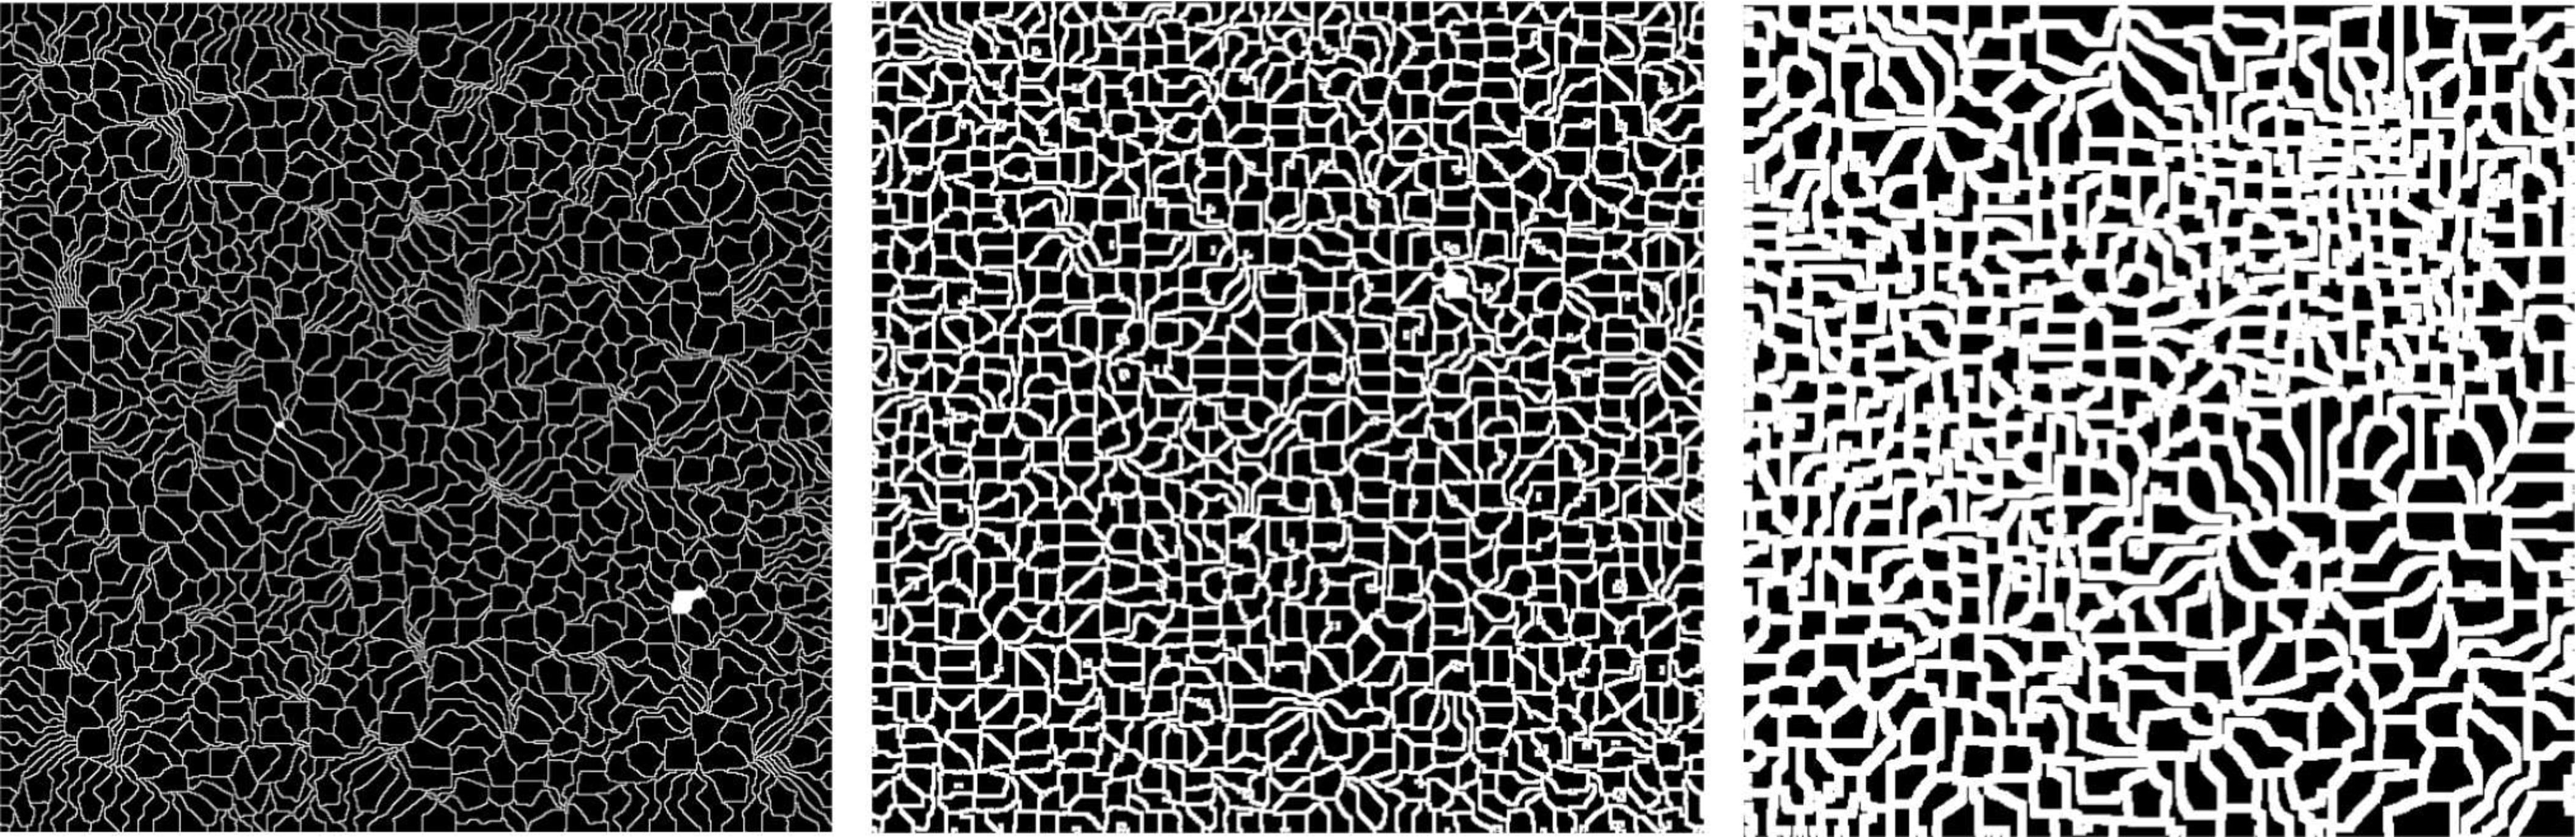
\includegraphics[scale=0.22]{fig1.pdf}}
  \caption{Diferentes separaciones entre part\'iculas utilizando el par\'ametro tama\~no del contorno. Izquierda: separaci\'on = 1, centro: separaci\'on = 2, derecha: separaci\'on = 4.}
  \label{fg:fig1}
\end{figure*}

Finalmente, el algoritmo devuelve la grilla $L$, la cual ser\'a renderizada posteriormente. En la siguiente secci\'on se explica la utilizaci\'on de sistemas din\'amicos en la evoluci\'on guiada de part\'iculas.

\subsection{Sistemas Din\'amicos}

La din\'amica es el estudio del {\em cambio}. Los estudios en din\'amica comenzaron en siglos previos con Isaac Newton. Las ecuaciones diferenciales son un resultado de sus estudios. Las mismas fueron disen\~nadas con el prop\'osito de tratar con la dificultad (o imposibilidad) de hallar soluciones anal\'iticas para determinados procesos din\'amicos. En primer lugar, se define un modelo matem\'atico del problema, del cual luego las ecuaciones diferenciales asociadas son obtenidas. La evoluci\'on del sistema es simulada y soluciones aproximadas son obtenidas en cada paso de la simulaci\'on. Estos sistemas tratan procesos que evolucionan con el tiempo, como la econom\'ia, la transferencia de calor, o el clima.

Los sistemas de ecuaciones diferenciales asociados son resueltos por medio de aproximaciones num\'ericas en cada instante de tiempo. El desarrollo de las computadoras en el \'ultimo siglo ha hecho posible que la disciplina se desarrolle en campos donde antes resultaba imposible como por ejemplo Fractales \citep{Mandelbrot83} y Caos.

Los costos computacionales de estas soluciones dependen de la complejidad del problema y el n\'umero de ecuaciones del sistema. En este trabajo proponemos usar un sub-\'area de ecuaciones diferenciales, llamadas ecuaciones diferenciales ordinarias (ODE). En esta representaci\'on, el tiempo es tratado como la \'unica variable independiente.


De manera general, las ODEs se representan utilizando el siguiente sistema de ecuaciones:
\begin{equation} \label{eq:simple}  
  \begin{aligned}
    \dot{x_{1}} = f_{1}(x_{1},\ldots,x_{n}),\\
    \ldots\\
    \dot{x_{n}} = f_{n}(x_{1},\ldots,x_{n}),
  \end{aligned}
\end{equation}

\noindent donde $\dot{x_{i}}$ representa la derivada de $x_{i}$ con respecto
a $t$. Las variables $x_{i}$ y las funciones $f_{i}$ son definidas de manera diferente para cada problema. En este caso, cada variable representa una coordenada cartesiana en el espacio, {\em i.e.,} $x_{1}$ es $x$, $x_{2}$ es $y$ y $x_{3}$ es $z$. El conjunto de $f_{i}$ ser\'a definido tratando de capturar la estructura interna del pan. La siguiente secci\'on muestra como estos sistemas pueden describir la evoluci\'on de los sistemas de part\'iculas.

\subsection{Evoluci\'on de sistemas de part\'iculas utilizando sistemas din\'amicos}

La percepci\'on humana puede detectar patrones en la estructura de la miga de pan. Distintas observaciones pueden realizarse sobre la distribuci\'on de las burbujas en la misma (ver Fig.~\ref{fg:fig2}). Primero, la forma de las burbujas cercanas a la corteza tiende a estirarse paralelamente a la misma. Esto es resultado de la acci\'on de las elevadas temperaturas durante la cocci\'on de la masa. Tambi\'en resulta evidente que la estructura completa es similar a un fluido con la forma de la corteza.


\begin{figure*}[htb!]
  \centerline{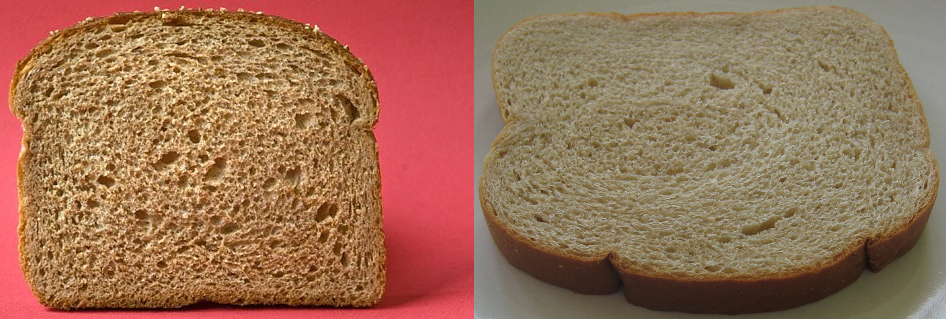
\includegraphics[scale=0.45]{fig2}}
  \caption{Im\'agenes de cortes reales de pan}
  \label{fg:fig2}
\end{figure*}

Por otro lado, los sistemas din\'amicos previamente presentados producen formas naturales (ver Fig.~\ref{fg:fig3}). En las im\'agenes pueden observarse c\'irculos y espirales, entre otras formas. Las im\'agenes fueron obtenidas dibujando trayectorias sobre un plano, siguiendo distintas ODEs. Tres ODEs describen las din\'amicas presentes en las im\'agenes. A modo de ejemplo, la imagen de la izquierda es producida por el siguiente conjunto de ecuaciones:

\begin{equation} \label{eq:simple}  
  \begin{aligned}
    \dot{x} &= x^{2}-y^{2}+1,\\
    \dot{y} &= 2xy+1.
  \end{aligned}
\end{equation}


\begin{figure*}[htb!]
  \centerline{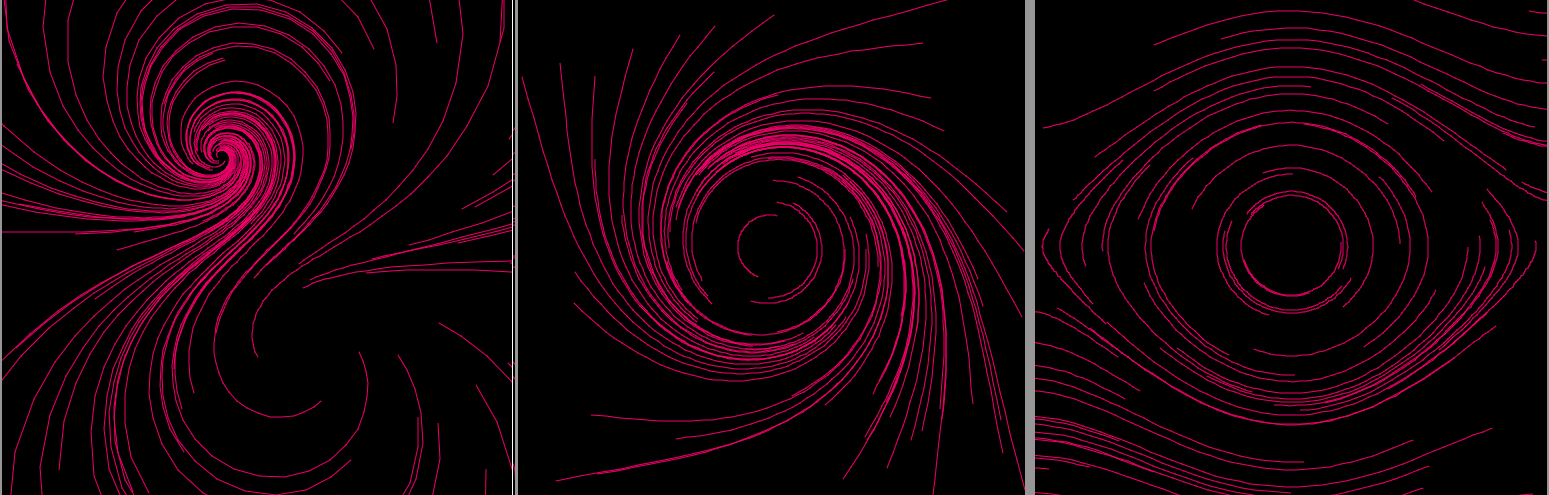
\includegraphics[scale=0.28]{fig3}}
  \caption{Sistemas din\'amicos en el plano.}
  \label{fg:fig3}
\end{figure*}

Posiciones aleatorias son elegidas en los ejemplos. Luego, el sistema es resuelto por medio de un {\em solver} Runge-Kutta de cuarto orden, el cual permite conocer la direcci\'on a tomar en cada punto por la trayectoria (en las im\'agenes adem\'as se utilizaron pasos negativos de tiempo para lograr una mejor visualizaci\'on). La imagen de la izquierda muestra un atractor y un repulsor claramente visibles. El centro de la espiral m\'as a la izquierda es un atractor (a medida que $t$ avanza, las trayectorias convergen hacia el punto), mientras que el otro centro es un repulsor. Los atractores pueden no ser puntuales, como muestran las restantes dos im\'agenes. La imagen de la derecha muestra atractores en forma de c\'irculos (las trayectorias ciclan por el c\'irculo).

Patterns can be produced by particles following trajectories in the plane or space. In order for a particle to follow a trajectory, the dynamical system is solved at the current position of the particle, and the contour position which best approximates that solution is chosen for growing. In other words, the dynamical system defines a vector field that could be used by the particles.

When the particles' growing direction is set to follow this vector field, bubbles are globally deformed in a similar shape as the
trajectories of the dynamical system (see Fig.~\ref{fg:fig4}). In the
images, from left to right, the trajectories' {\em randomness} is decremented. The right image was produced with randomness set to $0.1$, meaning
that the bubbles are forced to follow the dynamical system
trajectories with a probability of 0.9. This probability is defined as
$1-randomness$, with $0 \leq randomness \leq 1$. The dynamical system
used is the same as the right image shown in Fig.~\ref{fg:fig3}.  The
patterns are adequate for use not only in bread images, but also
cakes, and other baked foods, varying the randomness
parameter. Different useful structures could be defined by different set of equations and different parameters for the
particle systems (lifetime of particles, randomness).


\begin{figure*}[htb!]
  \centerline{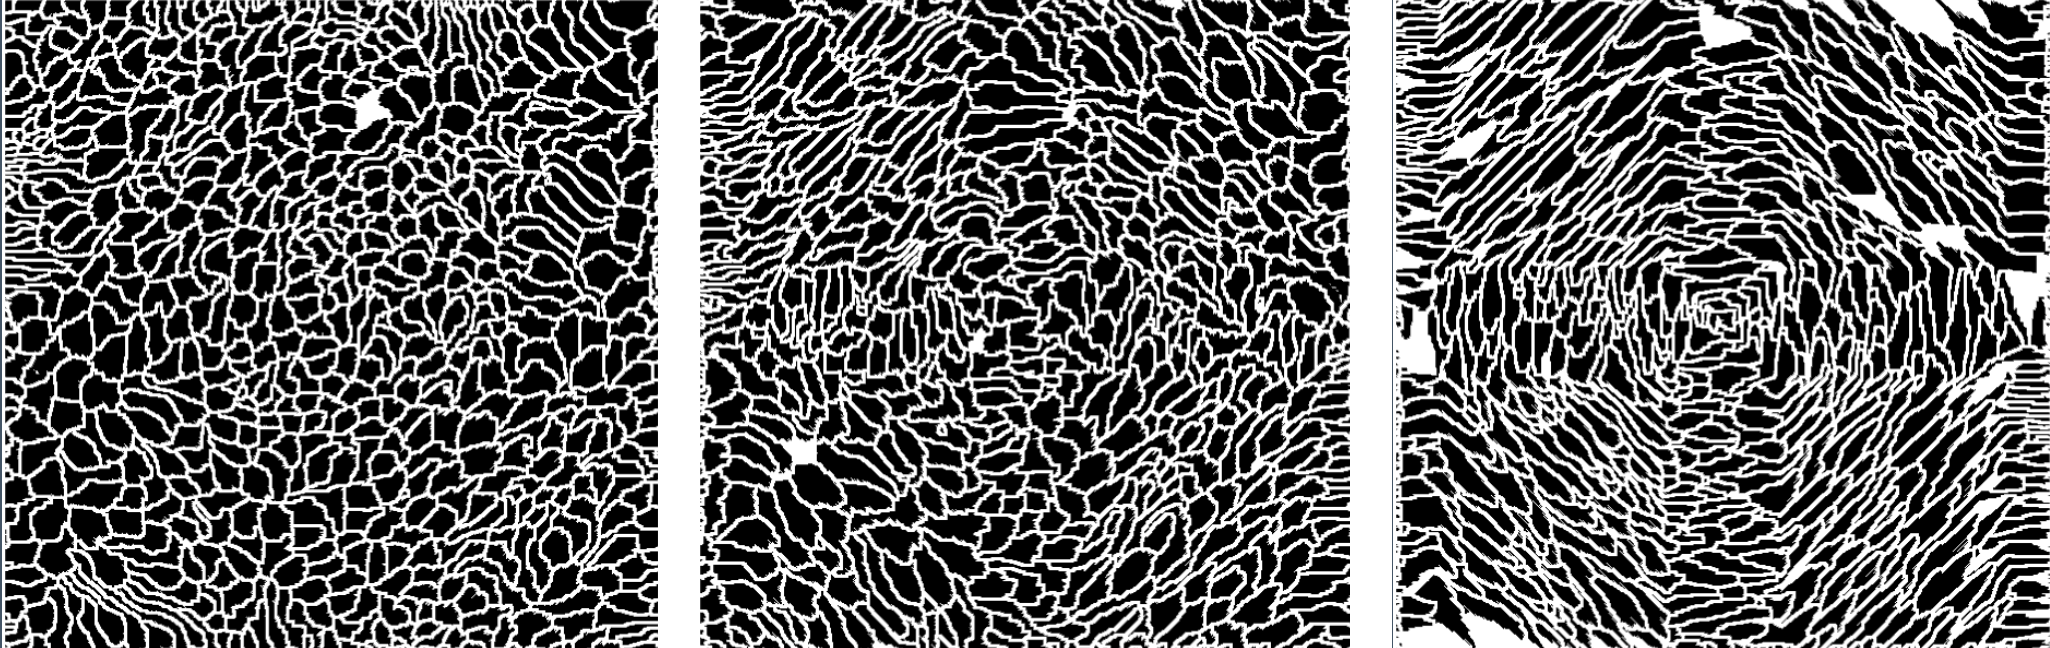
\includegraphics[scale=0.21]{fig4}}
  \caption{Dynamical systems affecting particle systems. Effect of the randomness parameter. From left to right, randomness: 0.3,0.2,0.1 respectively. }
  \label{fg:fig4}
\end{figure*}

The next section shows how these evolved particles can be rendered.

\subsection{Rendering algorithm}

In this section, the theory and implementation of the DVR algorithm used in this work is exposed.

\subsubsection{Direct volume rendering}

The technique of direct volume rendering attempts to provide a
2-dimensional representation of a volume defined by a discrete
3-dimensional density function. Rays are casted from the point of view
of a camera in a virtual scene and the density function is used to
compute the amount of light that the camera receives from the
direction of that ray. This is done by sampling the density function
along the ray in order to approximate the effect of different light
phenomena such as extinction, transmittance and scattering among
others. The lighting information gathered from these rays is then
used to compute the colour of the pixels in the final image.

Radiance is the amount of light that passes, or is emitted, from a
point and falls within a given solid angle. In the context of DVR, the
media that the rays traverse are taken as emissive, so when inspecting
the amount of light received for a given ray, what we are really doing
is approximating the radiance received from a distant point along the
direction of the ray. The radiance value is approximated by the
addition of the background radiance and the radiance emitted by the
media along the direction of the ray \citep{Kratz2006} : 

\begin{equation} \label{eq:general_radiance}  
  L(p_n) = L_b + \int_{p_0}^{p_n} \frac{\partial L(t)}{\partial p} \, dt,
\end{equation}

\noindent where $L_b$ is the background radiance, $p_0$ and $p_n$ are the
closest and furthest visible points along the ray direction,
respectively, $L(t)$ is the radiance sampled at point $t$, and
$\partial p$ is the distance between sampled points. For the purposes
of computing $L(p_n)$, the integral is approximated by a sum.

Extinction is the loss of photons in a ray shaft due to absorption in
the participating media and scattering to other directions. Some of
the photons will collide with the particles in the
surrounding media and be absorbed and transformed to energy, mostly
heat. Others will bounce and move along other directions. This is
approximated by using an absorption coefficient for the media, $k_a$
and a scattering coefficient $k_s$. If the scattering effect is
neglected, the formula for the amount of radiance absorbed over a
ray segment is:

\begin{equation} \label{eq:radiance_absorption}  
    L_b \ \displaystyle e^{-\int_{p_0}^{p_n} k_a(t) \, dt}.
\end{equation}

The value $\int_{p_i}^{p_j} k_a(t) \, dt$ is called the
absorption coefficient and referred to as $\tau_{(p_i, p_j)}$.

Transmittance is a complementary concept to extinction, and describes
the amount of light that passes through a media in a given
direction. The value of transmittance along two points $p_i$ and $p_j$
is:

\begin{equation} \label{eq:general_radiance}  
  T(p_i,p_j) = e^{-\tau_{(p_i, p_j)}}.
\end{equation}

If light emission is assumed to be a constant term ($\rho$) for
every point in the volume, our initial radiance estimate becomes:

\begin{equation} \label{eq:ray_radiance}  
  L(p_n) = L_b \ e^{-\tau(p_0, p_n)} + \int_{p_0}^{p_n} \rho \ e^{-\tau(t,p_n)} \, dt.
\end{equation}

This means that the radiance along points $p_0$ and
$p_n$ is the remaining background radiance after attenuation plus the
emission at every point in the ray, also attenuated.

DVR defines a volume inside which to sample a density function at
regular intervals and uses that information to approximate the
transmittance along those points and compute the amount of light
reaching the camera along the direction of a ray. The integral sum is
replaced by a discrete sum over the length of the ray that intersects
the volume.

Other effects can be accounted for, which augment the fidelity of the
final image, as well as the computing cost of the technique. Some of
these effects are phase, incidental scattering, and
out-scattering. Since the goal of this work is to achieve real time
frame rates, the basis of our rendering algorithm uses the simplified
transmittance only model.

\subsubsection{Implementation}

\paragraph{Overview}

In order to test the particle system used to describe the structure of
the bread, a demo application was created\footnote{available at
  \emph{\url{https://www.github.com/rbaravalle/Pysys}}} that uses the particle
system described to generate a volume texture. This volume texture is
then used to shade a cube with a DVR based shader. This demo shows
that the proposed method is compatible with current
rasterization-based real-time GPU rendering pipelines, providing a
realistic looking material, as well as shadow-map based real-time
shadows. This means that the material techniques proposed in this
article  can easily be integrated into any shader-based 3D engine with
minimal modifications.

\paragraph{Details}

The mesh defined for the model employing our DVR-based material is a unit
cube. The vertex shader code is very simple, providing only geometry
information to the fragment shader, which does the bulk of the
computations. 

Firstly, a ray is computed with the fragment position as origin and
the direction from the camera position to the fragment as the ray
direction. This ray is then traversed at regular intervals, sampling
the volume texture that represents the density of the bread. This
density is used to compute the accumulated transmittance from the ray
origin to the sample point. Once the transmittance falls below a
threshold value or the ray exits the cube, the computation ends.

At each sampled point the transmittance in the direction of the light
source is also computed in a similar way: a ray is created from the
sample point to the light source. This information is used to
approximate the amount of light reaching the sample point, and it
allows to perform self shadowing within the model in a natural
way. 

The transmittance information of the ray sample points and the
lighting information is then used to shade the pixel. At this point,
different artistic considerations can be applied to yield different
looking materials. In the case of the sample images presented
in this work, the shading is done by assigning a darker colour to areas
considered to be the crust of the bread, and a soft yellowish colour is
assigned to the crumb parts. A very faint specular component is also
used. The lighting term obtained from computing the transmittance
towards the light provides the details of the structure.

Our demo allows us to modify parameters such as the
transmittance coefficient of the bread, the transmittance threshold,
the colour assigned to the crumb and the addition of a specular
highlight, among other effects. This has the additional consequence of
being able to produce images that resemble other porous materials,
such as sponges. In the next section, the results of these processes
are shown and discussed.

\section{RESULTS AND DISCUSSION}

In this section, different rendering results and computing times are shown. A brief discussion is also outlined.

\subsection{Rendering results}

This section shows different images obtained with the proposed
method. The hardware employed is a nVidia GTX 480 ($480$ cores), which
is a typical configuration for home computers. The CPU is an Intel(R)
Core(TM) i5-2300 CPU (quad core). The screen resolution is
$1440\times990$ pixels. Different images with high bread resemblance
are obtained. Different bread types can be rendered varying colours
and transmittance parameters (see Fig.~\ref{fg:fig5}). In the middle
image, patterns produced by the particle system described in previous
sections can be clearly observed. In that case, the lifetime of the
particles is different from each other, in order to have big and small
bubbles at the same time. 

\subsection{Crust, slices and cuts}
A function defines whether a point in the volume is part of the crust
or part of the crumbs. For instance, a cylindrical bread could define
a position as crust if the point has certain distance to the centre of
the volume (in $X,Y$ coordinates, for all $Z$) , and crumb when its
distance is lower. Another function defines whether a point should be
considered empty air. This allows an easy way to define slices in the
bread. For example slices could be defined by returning true if the
modulus of the z coordinate division in the position vector with
certain number is $0$ (the width of the slice).  This produces prisms
of air in the volume which resemble slices as can be seen in the
images (see Fig.~\ref{fg:fig5}, \ref{fg:fig6}).

Since mathematical inequations based on positions should be written, this process should be extended to be ready to use by artists.

\begin{figure*}[htb!]
  \centerline{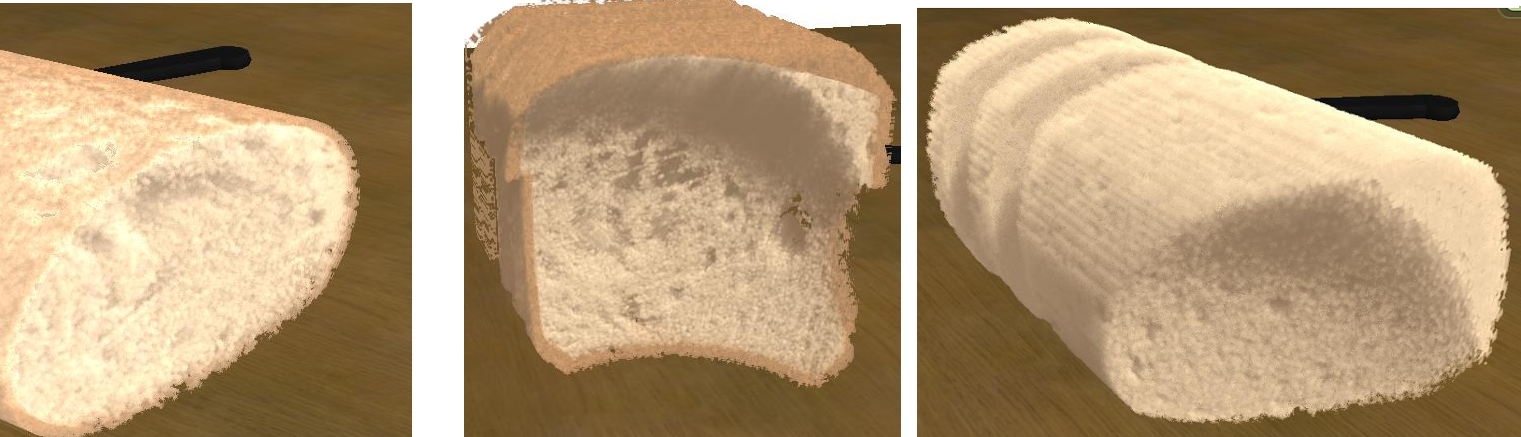
\includegraphics[scale=0.3]{fig5}}
  \caption{Different breads rendered in real time with the method described in this paper. The right image shows a bread which has no crust. }
  \label{fg:fig5}
\end{figure*}

Other materials could also be synthesised (see
Fig.~\ref{fg:fig6}). They are the result of varying different
parameters of the model. In the image, a sliced pudding (left) a slice
of cake (middle) and a sponge (right) are rendered. They have been
easily derived by changing the colour of the volume, and the structure,
in the case of the sponge. When no living yeast are involved in the
manufacturing process, a random volume texture could be used. Back
illumination is also present in the model (see Fig.~\ref{fg:fig7}). In
the figure, a sponge is illuminated from behind and light propagation
in its medium is seen.

\begin{figure*}[htb!]
  \centerline{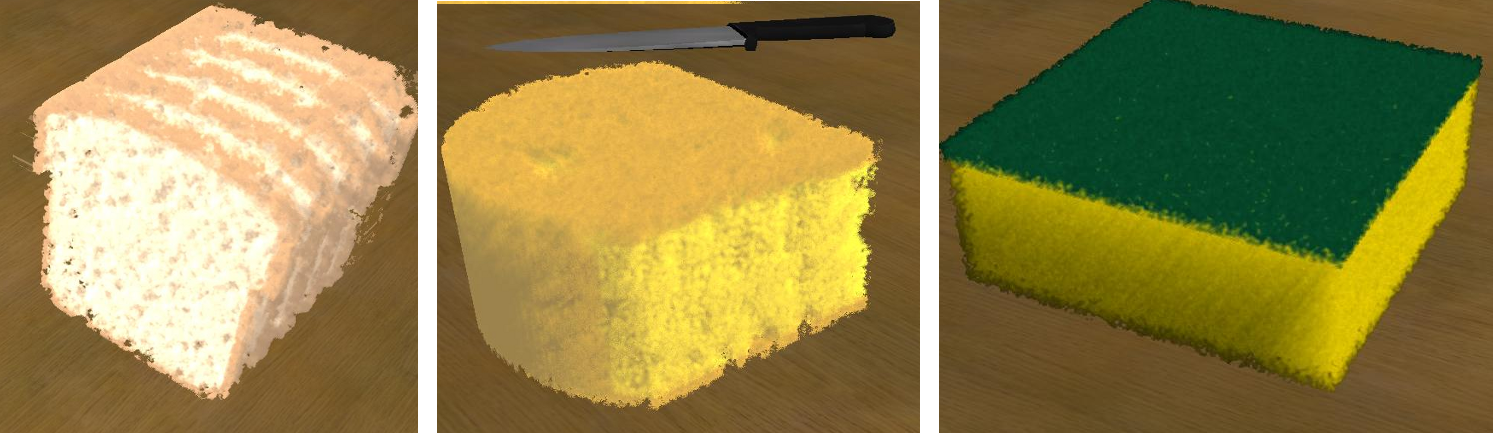
\includegraphics[scale=0.3]{fig6}}
  \caption{Other materials rendered in real time changing parameters in the model. Left: sliced pudding, middle: slice of cake, right: sponge. }
  \label{fg:fig6}
\end{figure*}



\begin{figure*}[htb!]
  \centerline{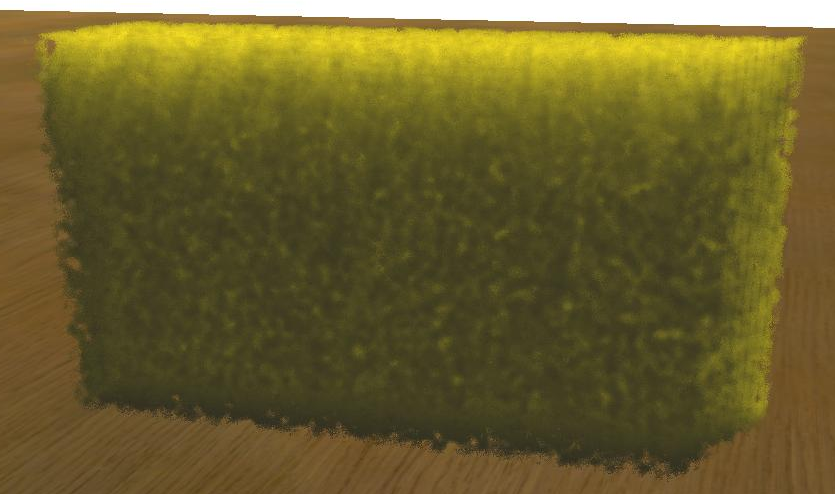
\includegraphics[scale=0.25]{fig7}}
  \caption{Sponge showing back illumination in the model. }
  \label{fg:fig7}
\end{figure*}


\subsection{Computing times}
Most images show real time results (FPS over 30), see Table~\ref{tab:n1} . The performance is affected mostly when the transmittance is low ({\em i.e.}, when the material becomes more transparent), since the ray accumulates more information (and the computation ends later). Another key parameter are the steps that a ray traverses. We experimentally found that values above $100$ steps give reasonably images in all cases. The process automatically scales with the number of GPU processors, so the fps count will increment in the GPUs of the next years.

\begin{table}[htb]
\centering
\begin{tabular}{|c|c|c|c|c|c|c|}
\hline &  Bread 1 & Bread 2 & Bread 3 & Pudding & Cake & Sponge \\
\hline
\hline
 mean FPS  & 32.2 &  75.5 &  45.2 & 28.5 &  54.2 & 29.7\\
\hline
 Steps &  140 &  140 &  140 & 256 &  140 & 256 \\
\hline
 Transmittance &  15 &  15 &  15 & 15 &  15 & 2.25 \\
\hline
\end{tabular}
\caption{Computing times and key parameters for the images obtained. }
\label{tab:n1}
\end{table}

\subsection{Discussion}
To the best of the authors knowledge, this is the first attempt to convincingly render bread crumb in real time without introducing complex intermediate processes (capture, mesh generation, precomputation, post-process). It is true that a previous approach \citep{Cho2007} has been used for bread rendering, but comparisons with this technique could not be established since no details are explained (computing times, render method).

Different regions with different parameters in the volume can be
defined, and this idea is used to show crumb and crust of different
colour parameters. 
%% Also, since entire regions of the volume could be
%%changed, the approach can be used in a simulation where a knife cuts
%%slices of bread. 
Integration with shader based engines is easily managed. Depth
information from fragments can be obtained, so it can be naturally
integrated in scenes, as the different images shows.

Computing times show an excellent performance which depends mostly on
the number of steps and the transmittance chosen. Nevertheless, real
time rates are always reached except when it encompasses a big portion
of the screen, since the approach is largely fragment-shader bound. In
years to come, this method will automatically augment its fps count
since it scales with the number of processors.

The promising results obtained can be extended in number of ways,
outlined at the end of this paper.


%\section{CONCLUSIONS AND FUTURE WORK}


%\subsection{Main headings}

%The main headings should be written left aligned, in 12pt, boldface
%and all capital Times Roman letters. There should be a 12pt space
%before, and 6pt after the main headings.

%\subsection{Secondary headings}

%The secondary headings should be written left aligned, in 12pt,
%boldface Times Roman, with an initial capital for first word only. There
%should be a 12pt space before, and 6pt after the secondary headings.

%\section{TEXT}

%The normal text should be written single-spaced, justified, using 12pt
%Times Roman in one column. The first line of each paragraph must be
%indented 0.5cm. There is not inter-paragraph spacing.

%\section{PAGE NUMBERS}

%The authors {\bf must not number} the pages of the article. Numbers will
%be added by the editor/publisher. 

%\section{FIGURES}

%All figures should be numbered consecutively and captioned. The
%caption should be written centered, in 10pt Times Roman, upper and lower
%case letters.

%\begin{figure*}[htb]
%\centerline{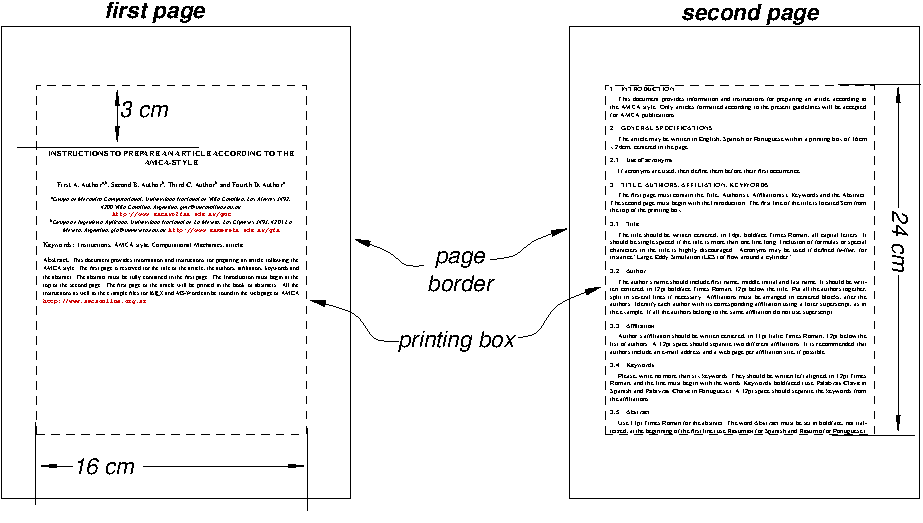
\includegraphics{firstpage}}
%\caption{Page layout}
%\label{fg:figure}
%\end{figure*}

%A 6pt space should separate the figure from the caption, and a
%12pt space should separate the upper part of the figure and the
%bottom of the caption from the surrounding text (see
%Fig.~\ref{fg:figure}).

%Figures should be referenced in the text. Color figures are welcomed.

%\section{EQUATIONS}

%A displayed equation is numbered, using Arabic numbers in parentheses.
%It should be  centered, leaving a 6pt space above and below to separate it from
%the surrounding text.

%The following example is a simple single line
%equation
%
%\begin{equation}
%Ax = b.
%\end{equation}

%The next example is a multi-line equation
%
%\begin{equation} \label{eq:simple}  
%\begin{aligned}
%Ax& = b,\\
%Ax& = c.
%\end{aligned}
%\end{equation}
%
%If possible, internal PDF links must be generated for references to
%equations. The recommended color for links to references in the text
%is blue (e.g., see Eq.~(\ref{eq:simple})).

%\section{TABLES}

%All tables should be numbered consecutively and captioned, the caption
%should be 10pt Times Roman, upper and lower case letters.

%A space of 6pt separates the table from the caption, and 12pt space
%separates the table from the surrounding text. For an example, see
%Table~\ref{tab:n50}. Tables should be referenced in the text.

%\begin{table}[htb]
%\centering
%\begin{tabular}{|c|c|c|c|}
%\hline  & 20x20 mesh & 50x50 mesh & 100x100 mesh\\
%\hline
%\hline
% 0 & 41.00 & 1.00 & 4.92\\
%\hline
% 1 & 40.86 & 1.02 & 4.88 \\
%\hline
%10 & 23.81 & 3.44 & 2.92 \\
%\hline
%50 & 5.62 & 64.20 & 1.08 \\
%\hline
%\end{tabular}
%\caption{Condition number for the Stekhlov operator. }
%\label{tab:n50}
%\end{table}

%\section{FORMAT OF REFERENCES}

%References should be quoted in the text using the \emph{author-style}
%(a.k.a. \emph{Harvard style}). References can be cited in
%\emph{parenthetical} form \citep{zienkiewicz91,idelsohn94,meyer82,meyer82b}, or
%in \emph{textual} form, e.g. see
%\citet{zienkiewicz91,idelsohn94,meyer82,meyer82b}.  References are grouped
%together and sorted alphabetically at the end of the article as shown
%in these instructions. Do not include references that are not cited in
%the article body. 

%If possible, internal PDF links must be generated for citations. The
%recommended color for links to references in the text is blue. The
%preferred color for links to external references, as web pages, 
%is red (e.g. \url{http://www.amcaonline.org.ar}).

\section{CONCLUSIONS}

In this paper the transmittance model of DVR is applied in the GPU to a 3D scalar field representing the bread crumb structure, to obtain realistic bread crumb images. This structure is generated using particle systems in which particles follow dynamical systems in a probabilistic way. A numerical simulation is employed to solve the resulting set of equations which represents the dynamical system. Results show high fidelity images in real time, suitable for application in several areas, such as serious games \citep{Susi2007} and photo-realistic rendering. This procedure does not present the drawbacks of other state of the art methods, such as capture processes or mesh generation.

The main disadvantage of the method is resolution, since close look-ups of the structure could lead to homogeneous areas due to hardware constraints, {\em i.e.}, arbitrary texture sizes are not allowed. This disadvantage is not exclusive of our method. A number of possible solutions will be employed to overcome this problem, such as setting different volume textures depending on the distance to the volume. 

As possible continuations of this work, DVR could be extended to handle other phenomena such as indirect illumination and sub surface scattering in order to enhance the images obtained. Also, partial differential equations will be employed to implement the baking process of bread \citep{Purlis2012}. Other porous materials such as cheeses will be investigated. Another interesting work will be to define primitives for crumb and crust modelling (shapes and intersections), enabling artists to define its shape.

%Template files in TeX, \LaTeX{} and MS-Word may be found at the
%AMCA web site: \url{http://www.amcaonline.org.ar}. 
%Remember: {\bf Do not number the pages.}
%
\bibliography{eniefbib}
\end{document}
% $Id: amcapaper.tex,v 1.23 2006/08/14 16:58:45 mstorti Exp $
